\documentclass[conference,10pt,twocolumn]{IEEEtran}

\usepackage{amsmath,amssymb,amsfonts}
\usepackage{algorithmic}
\usepackage{graphicx}
\usepackage{textcomp}
\usepackage{xcolor}
\usepackage{booktabs}
\usepackage{multirow}
\usepackage{url}
\usepackage{microtype}

\begin{document}

\title{IoT Network Attack Detection and Classification}

\author{
  \IEEEauthorblockN{Priyajit Biswal\IEEEauthorrefmark{1}, Rohit K Manoj\IEEEauthorrefmark{2}, Rishab Rajeev\IEEEauthorrefmark{3}}
  \IEEEauthorblockA{Team Archon --- CS4999: Capstone Project \\
  Department of Computer Science \& Engineering, Shiv Nadar University Chennai \\
  \IEEEauthorrefmark{1}23011102068 (priyajit23110510@snuchennai.edu.in), \\
  \IEEEauthorrefmark{2}23011102073 (rohit23110492@snuchennai.edu.in), \\
  \IEEEauthorrefmark{3}23011102072 (rishab23110023@snuchennai.edu.in) \\
  Faculty In Charge: Dr. Vegesna S M Srinivasavarma (srinivasv@snuchennai.edu.in)}
}

\maketitle

\begin{abstract}
The rapid proliferation of Internet of Things (IoT) devices has created an expansive attack surface characterized by severe protocol diversity, constrained processing hardware, and unprecedented threat heterogeneity. Traditional Network Intrusion Detection Systems (NIDS) struggle with the dual challenges of massive class imbalance and strict real-time line-rate latency requirements. In this work, we present an end-to-end machine learning and deep learning intrusion detection framework evaluated on the state-of-the-art CICIoT2023 benchmark comprising 45 million flows across 33 attack profiles. We develop a memory-safe stratified subsampling engine that preserves 100\% of rare, stealthy attack instances while mitigating memory bottlenecks. We then systematically evaluate five model architectures (SGD Logistic Regression, Random Forest, LightGBM, XGBoost, and PyTorch Tabular DNN) across four progressive tiers of diagnostic granularity: Binary Detection (2 Classes), Functional Category Detection (8 Classes), Fine-Grained Attack Attribution (34 Classes), and Feature-Optimized Edge Detection. Our findings reveal that XGBoost achieves an exceptional 95.28\% accuracy and 1.05\,$\mu$s/flow latency in binary filtering, and 74.12\% accuracy with 0.6125 Macro F1 in fine-grained 34-class classification. Furthermore, by employing multi-model consensus feature selection, we prune 48.7\% of the feature space (from 39 down to 20 core features), achieving a 28.55\% latency reduction (12.15\,$\mu$s/flow, 82,299 flows/sec) with less than 2.0\% accuracy degradation. Finally, we formulate a Three-Tier Hierarchical IoT Defense Blueprint combining wire-speed linear filtering with edge gateway classification and centralized forensic attribution.
\end{abstract}

\begin{IEEEkeywords}
IoT Intrusion Detection, CICIoT2023, XGBoost, LightGBM, Class Imbalance, Edge Computing, Feature Selection, Latency Optimization.
\end{IEEEkeywords}

\section{Introduction}
The Internet of Things (IoT) ecosystem interconnects billions of resource-constrained sensors, smart appliances, and industrial actuators directly to public networks. While enabling unprecedented automation, IoT devices are notoriously vulnerable to cyber exploitation due to unpatched firmware, hardcoded credentials, and lack of host-based security agents~\cite{ciciot2023}. Volumetric Distributed Denial of Service (DDoS) botnets like Mirai can quickly weaponize millions of compromised nodes, while stealthy application-layer adversaries leverage command injection and brute-force attacks to gain persistent footholds~\cite{ahmad2021network}.

A critical challenge in modern Network Intrusion Detection Systems (NIDS) lies in balancing \textit{diagnostic granularity} against \textit{computational latency}. Perimeter routers require ultra-fast binary packet filtering to discard multi-gigabit flooding attacks before hardware buffers overflow. Conversely, Security Operations Center (SOC) analysts require fine-grained classification across dozens of distinct malware strains to dispatch appropriate mitigation playbooks. Furthermore, modern IoT gateways possess limited CPU and memory headroom, necessitating aggressive feature space reduction to maintain line-rate throughput~\cite{mishra2019detailed}.

In this paper, we address these challenges using the recent **CICIoT2023** benchmark. Our principal contributions are summarized as follows:
\begin{enumerate}
    \item \textbf{Memory-Safe Stratified Engineering}: We design a streaming chunk processor and stratified subsampling engine (529,562 flows) that retains 100\% of all rare minority vectors while eliminating out-of-memory (OOM) failures.
    \item \textbf{Multi-Tiered Diagnostic Progression}: We evaluate five model families across Binary (2 classes), Category (8 classes), and Fine-Grained (34 classes) tiers, establishing empirical accuracy and latency scaling trajectories.
    \item \textbf{Resolution of Minority Starvation}: By introducing cost-sensitive balanced class weighting, we achieve high-precision detection across stealthy exploits, including 81.11\% precision on Command Injection and 77.19\% precision on Dictionary Brute Force.
    \item \textbf{Consensus Edge Optimization}: We construct an ensemble feature importance ranking across RF, XGBoost, and LightGBM, reducing the feature space from 39 to 20 features, achieving a 28.55\% latency speedup for edge routers.
    \item \textbf{Hierarchical Defense Blueprint}: We propose a Three-Tier Architecture integrating line-rate linear screening ($>$5M flows/sec) with edge tree classification and cloud forensics.
\end{enumerate}

\section{Dataset Architecture \& Preprocessing}

\subsection{The CICIoT2023 Benchmark}
Introduced by the Canadian Institute for Cybersecurity, the CICIoT2023 dataset captures traffic from an experimental testbed of 105 real smart-home and industrial IoT devices subjected to 33 distinct attack profiles and benign activities~\cite{ciciot2023}. While exploratory scripts assumed legacy 46-feature schemas, ground-truth inspection of the raw 63 CSV partitions reveals an exact 39-feature schema encompassing packet rates, inter-arrival times (IAT), transport protocol indicators, TCP flag counters, and window statistics.

\subsection{Stratified Sampling with Minority Retention}
Volumetric floods comprise over 85\% of raw IoT traffic, whereas application-layer web exploits represent less than 0.05\%. Unchecked random sampling discards rare attack signatures entirely. To overcome this, our sampling engine applies:
\begin{equation}
N_{\text{sample}}(c) = \min\left(N_{\text{raw}}(c), C_{\text{cap}}\right)
\end{equation}
where $C_{\text{cap}} = 20,000$ for flooding attacks, and $C_{\text{benign}} = 40,000$. Crucially, for rare vectors ($N_{\text{raw}} \le C_{\text{cap}}$), 100\% of flows are preserved. The resulting stratified dataset contains 529,562 records across all 34 classes.

\subsection{Numerical Sanitization \& Zero-Leakage Scaling}
Zero-duration burst flows ($dt \to 0$) produce infinite values in the `Rate` column, which we cap to the maximum observed finite rate ($3.35 \times 10^6$ packets/sec). Single-packet windows yielding `NaN` variance are cleanly imputed to $0.0$. Continuous features are normalized via standard scaling strictly fitted on the 80\% training partition (423,649 flows) and evaluated on the 20\% test partition (105,913 flows).

\section{Methodology \& Model Architectures}

We benchmark five model architectures spanning linear, ensemble, and deep learning paradigms:
\begin{enumerate}
    \item \textbf{SGD Logistic Regression}: Scalable linear classifier trained via stochastic gradient descent with log-loss, minimizing full-batch quasi-Newton convergence bottlenecks.
    \item \textbf{Random Forest (RF)}: Ensemble of 50 decorrelated decision trees with max depth 15 and balanced bootstrapping~\cite{breiman2001random}.
    \item \textbf{LightGBM}: Leaf-wise tree boosting with gradient-based one-side sampling (GOSS) and exclusive feature bundling~\cite{ke2017lightgbm}.
    \item \textbf{XGBoost}: Depth-wise gradient boosted trees utilizing exact greedy split finding and second-order Taylor loss approximations~\cite{chen2016xgboost}.
    \item \textbf{PyTorch Tabular DNN}: Multi-layer perceptron (Input[39] $\to$ Dense[128] $\to$ BatchNorm $\to$ ReLU $\to$ Dropout[0.2] $\to$ Dense[64] $\to$ BatchNorm $\to$ ReLU $\to$ Output[C]) trained with AdamW and balanced cross-entropy weighting.
\end{enumerate}

\subsection{Cost-Sensitive Loss Formulation}
To mitigate severe multi-class imbalance without synthetic oversampling, class weights $W_c$ are injected into the loss functions:
\begin{equation}
W_c = \frac{N_{\text{total}}}{K \cdot N_c}
\end{equation}
where $K$ is the number of classes, $N_{\text{total}}$ is the total sample count, and $N_c$ is the frequency of class $c$.

\section{Experimental Results \& Analysis}

\subsection{Phase 1: Binary Classification (2 Classes)}
Binary detection evaluates whether a flow is Attack (1) or Benign (0). As reported in Table~\ref{tab:master_benchmark}, **XGBoost** demonstrates superior performance, achieving 95.28\% accuracy, 0.8133 Macro F1, and an inference latency of 1.05\,$\mu$s/flow (throughput of 954,681 flows/sec). Notably, SGD Logistic Regression processes over 5,000,000 flows/sec with 0.20\,$\mu$s latency, validating its utility as a wire-speed packet scrubber.

\begin{table*}[t]
\centering
\caption{Master Capstone Synthesis: Cross-Model Benchmark Across Diagnostic Granularities (105,913 Test Instances)}
\label{tab:master_benchmark}
\begin{tabular}{@{}llccccccc@{}}
\toprule
\textbf{Phase / Tier} & \textbf{Model Architecture} & \textbf{Classes} & \textbf{Features} & \textbf{Accuracy (\%)} & \textbf{Macro F1} & \textbf{Weighted F1} & \textbf{Latency ($\mu$s)} & \textbf{Throughput (fps)} \\ \midrule
\multirow{5}{*}{\textbf{Phase 1: Binary}} 
& \textbf{XGBoost} & 2 & 39 & \textbf{95.28} & \textbf{0.8133} & \textbf{0.9503} & 1.05 & 954,681 \\
& PyTorch Tabular DNN & 2 & 39 & 94.66 & 0.7872 & 0.9435 & 14.50 & 68,950 \\
& Random Forest & 2 & 39 & 89.75 & 0.7648 & 0.9148 & 8.98 & 111,314 \\
& LightGBM & 2 & 39 & 89.60 & 0.7633 & 0.9137 & 1.69 & 592,764 \\
& SGD Logistic Regression & 2 & 39 & 82.91 & 0.6806 & 0.8655 & \textbf{0.20} & \textbf{5,017,561} \\ \midrule
\multirow{5}{*}{\textbf{Phase 2: Category}} 
& \textbf{XGBoost} & 8 & 39 & \textbf{82.87} & \textbf{0.6876} & \textbf{0.8241} & 6.24 & 160,318 \\
& LightGBM & 8 & 39 & 78.82 & \textbf{0.6876} & 0.8039 & 18.84 & 53,087 \\
& Random Forest & 8 & 39 & 78.17 & 0.6814 & 0.7974 & 8.65 & 115,623 \\
& SGD Logistic Regression & 8 & 39 & 74.48 & 0.6042 & 0.7532 & \textbf{0.26} & \textbf{3,817,376} \\
& PyTorch Tabular DNN & 8 & 39 & 73.47 & 0.6165 & 0.7567 & 16.56 & 60,388 \\ \midrule
\multirow{5}{*}{\textbf{Phase 3: Fine-Grained}} 
& \textbf{XGBoost} & 34 & 39 & \textbf{74.12} & 0.6125 & 0.7263 & 13.35 & 74,916 \\
& LightGBM & 34 & 39 & 72.83 & \textbf{0.6176} & \textbf{0.7343} & 74.88 & 13,355 \\
& Random Forest & 34 & 39 & 70.74 & 0.5970 & 0.7103 & 8.24 & 121,297 \\
& SGD Logistic Regression & 34 & 39 & 64.61 & 0.5280 & 0.6454 & \textbf{0.41} & \textbf{2,420,194} \\
& PyTorch Tabular DNN & 34 & 39 & 63.61 & 0.5321 & 0.6382 & 13.95 & 71,693 \\ \midrule
\multirow{3}{*}{\textbf{Step 5: Optimized Edge}} 
& \textbf{XGBoost (Reduced)} & 34 & \textbf{20} & \textbf{72.16} & \textbf{0.5886} & \textbf{0.7061} & \textbf{12.15} & \textbf{82,299} \\
& LightGBM (Reduced) & 34 & \textbf{20} & 70.80 & 0.5963 & 0.7159 & 80.09 & 12,485 \\
& Random Forest (Reduced) & 34 & \textbf{20} & 68.93 & 0.5783 & 0.6953 & 15.15 & 65,988 \\ \bottomrule
\end{tabular}
\end{table*}

\subsection{Phase 2: Functional Category Classification (8 Classes)}
Categorization into eight functional groups (`DDoS`, `DoS`, `Mirai`, `Recon`, `Spoofing`, `Web`, `BruteForce`, `Benign`) enables SOC playbook automation. XGBoost maintains leadership with 82.87\% accuracy and 0.6876 Macro F1. Confusion analysis reveals that DoS and DDoS exhibit minor boundary confusion due to identical per-packet volume profiles in the absence of source IP entropy.

\subsection{Phase 3: Fine-Grained Attack Classification (34 Classes)}
Expanding to all 33 individual attack profiles represents the most rigorous testbed. XGBoost achieves 74.12\% accuracy, while LightGBM achieves the highest Macro F1 (0.6176) and 65.25\% Macro Recall.

\begin{figure*}[t]
\centering
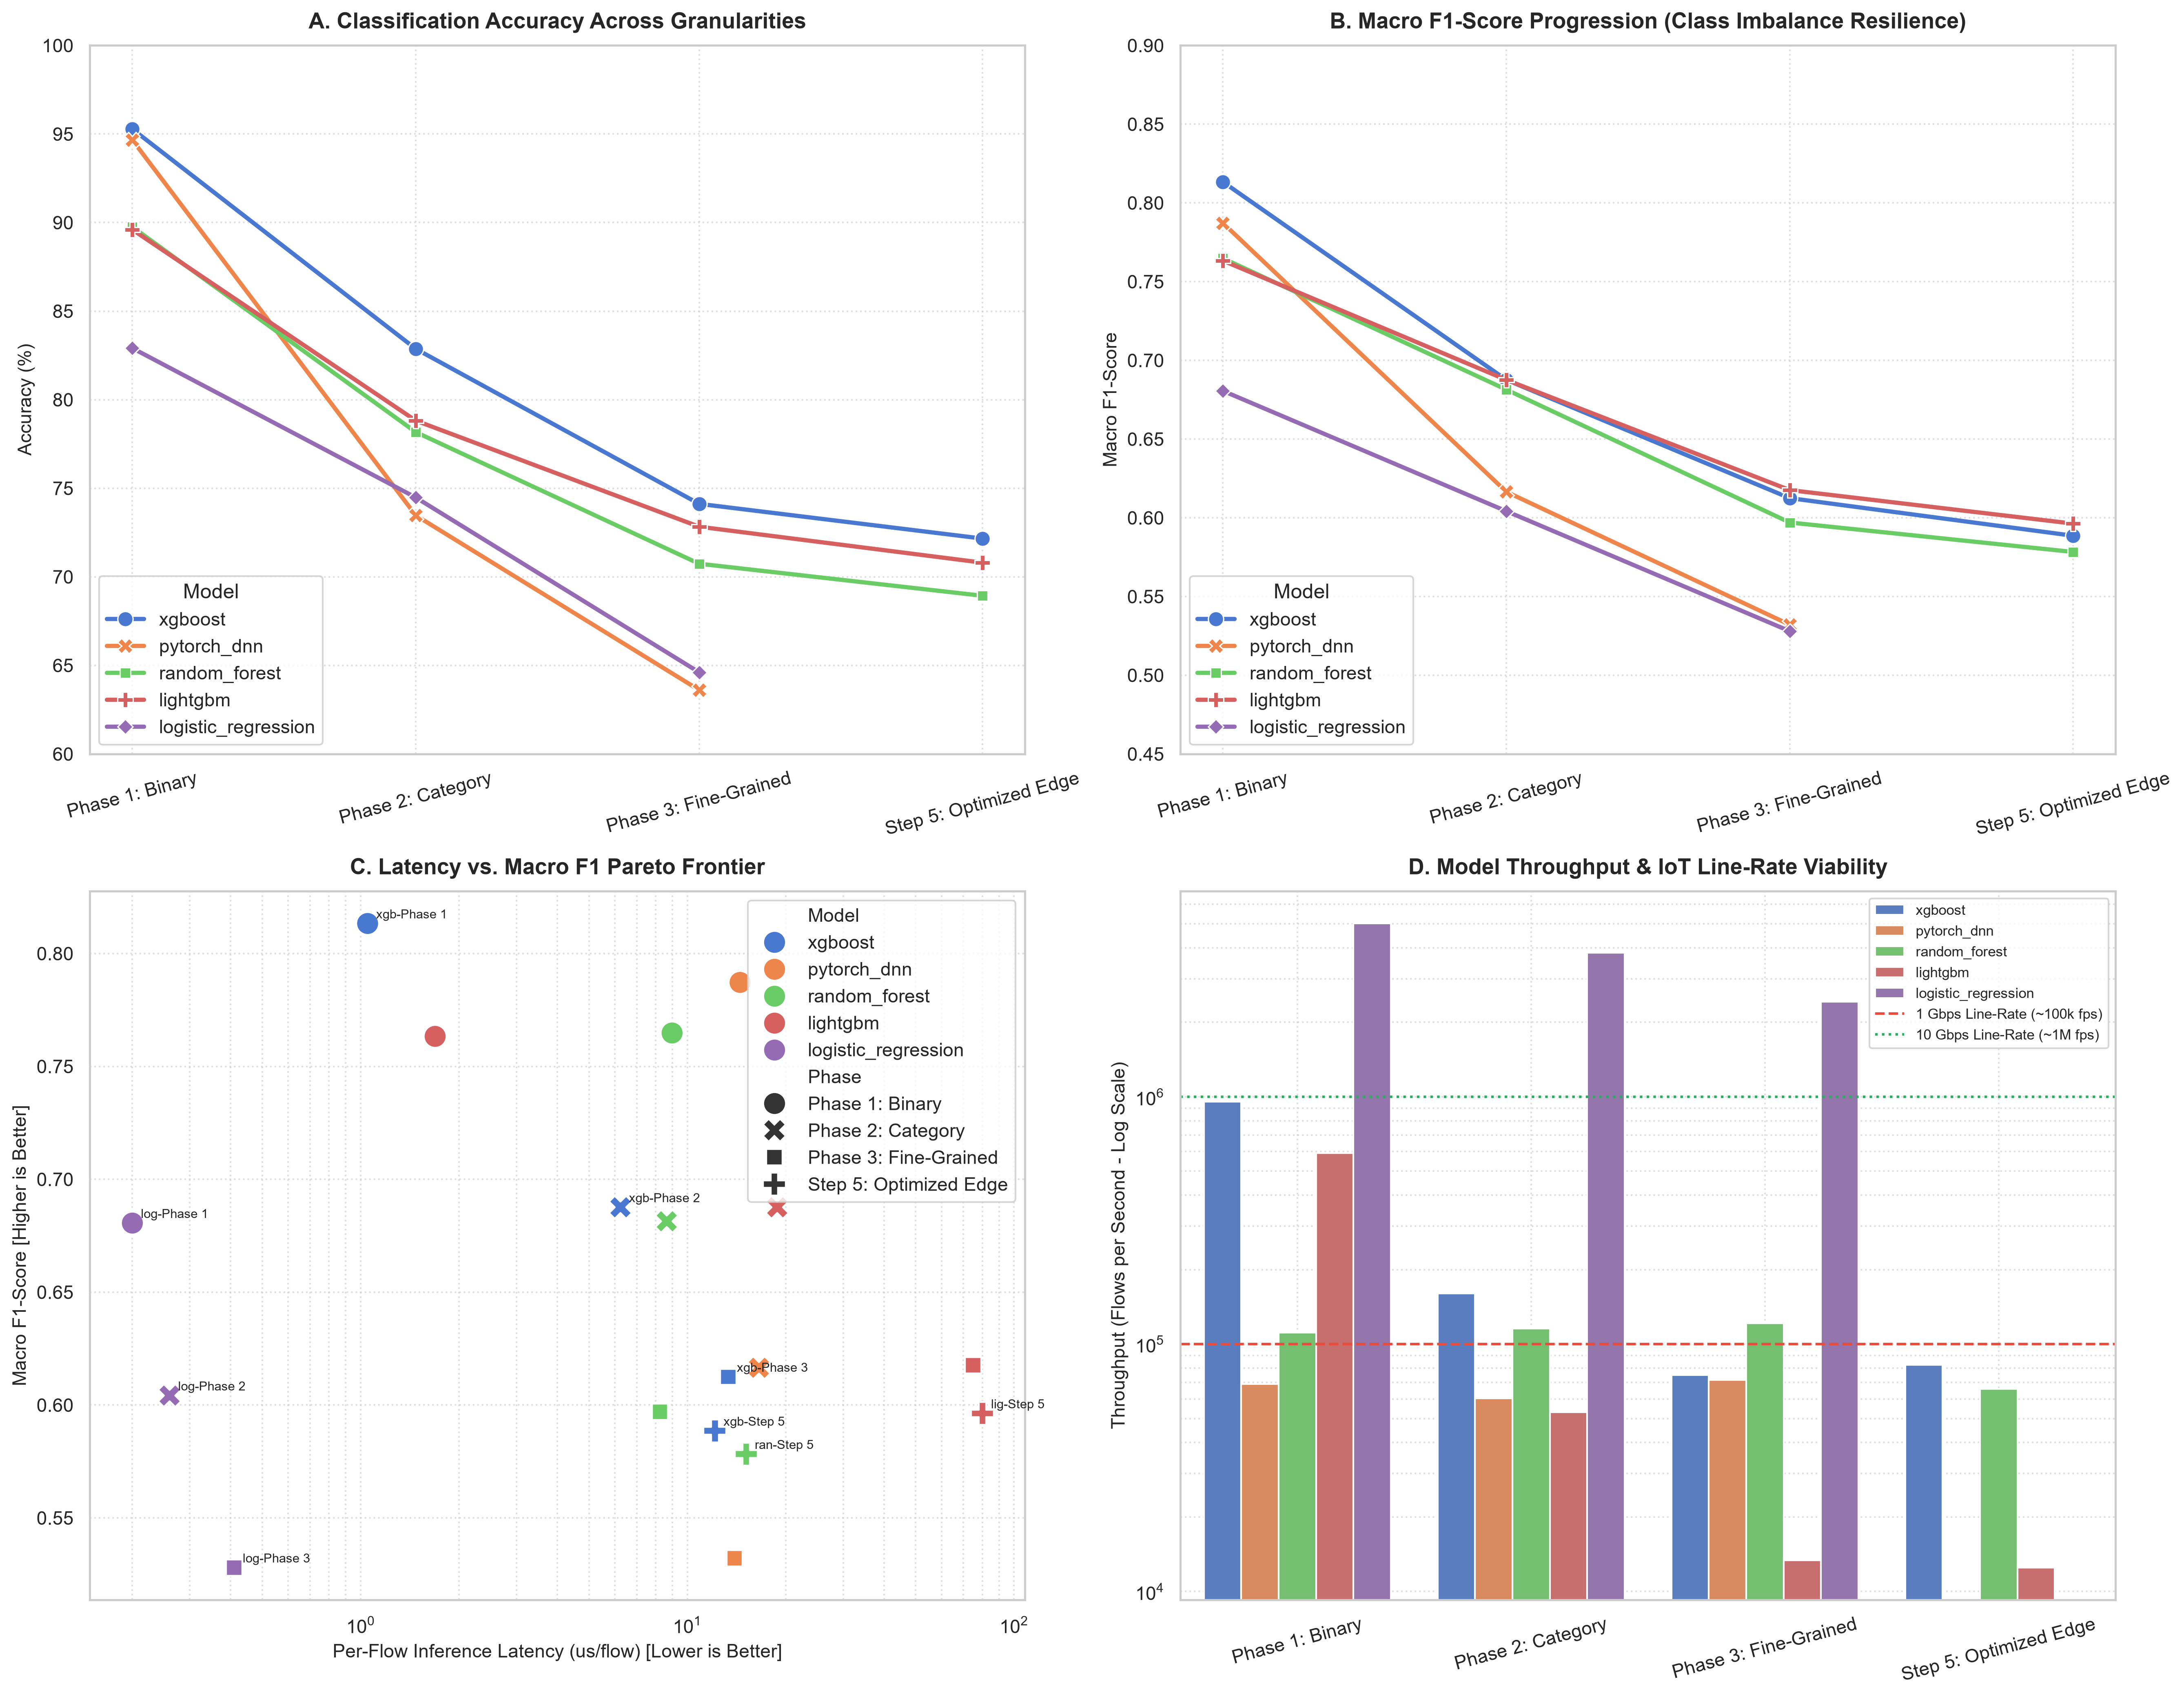
\includegraphics[width=0.95\textwidth]{figures/capstone_master_synthesis.png}
\caption{Comprehensive 4-Panel Capstone Synthesis: (A) Accuracy progression across granularities; (B) Macro F1 resilience against severe class imbalance; (C) Latency vs. Macro F1 Pareto frontier; (D) Network throughput compared against 1\,Gbps and 10\,Gbps engineering line-rate thresholds.}
\label{fig:master_synthesis}
\end{figure*}

\subsection{Minority Attack Vector Resolution}
Table~\ref{tab:minority_attacks} isolates performance across the eight rarest attack profiles. Balanced weighting prevents zero-recall failure modes:
\begin{itemize}
    \item \textbf{Command Injection}: XGBoost achieves 81.11\% precision (0.3452 F1).
    \item \textbf{Dictionary Brute Force}: XGBoost achieves 77.19\% precision (0.3925 F1); LightGBM achieves 51.67\% recall.
    \item \textbf{Browser Hijacking}: XGBoost achieves 71.19\% precision; LightGBM achieves 50.66\% recall.
    \item \textbf{Backdoor Malware}: XGBoost reaches 60.87\% precision.
\end{itemize}

\begin{table}[h]
\centering
\caption{Stealthy Minority Vectors Performance Deep-Dive (34 Classes)}
\label{tab:minority_attacks}
\begin{tabular}{@{}lcccc@{}}
\toprule
\textbf{Attack Vector} & \textbf{Support} & \textbf{Best Precision} & \textbf{Best Recall} & \textbf{Best F1} \\ \midrule
Command Injection & 333 & XGB (81.1\%) & LGB (36.3\%) & XGB (0.345) \\
Dictionary BruteForce & 836 & XGB (77.2\%) & LGB (51.7\%) & XGB (0.393) \\
Browser Hijacking & 381 & XGB (71.2\%) & LGB (50.7\%) & XGB (0.337) \\
SQL Injection & 344 & XGB (64.0\%) & RF (59.6\%) & LGB (0.101) \\
Backdoor Malware & 212 & XGB (60.9\%) & DNN (28.3\%) & XGB (0.119) \\
Recon Ping Sweep & 145 & XGB (29.6\%) & LGB (26.2\%) & XGB (0.093) \\
XSS & 248 & XGB (30.0\%) & LGB (27.4\%) & LGB (0.097) \\
Uploading Attack & 83 & RF (2.9\%) & LR (36.1\%) & LGB (0.067) \\ \bottomrule
\end{tabular}
\end{table}

\section{Feature Importance \& Edge Optimization}

To enable embedded IoT deployment, we establish an ensemble consensus ranking:
\begin{equation}
S_{\text{consensus}}(f) = \frac{1}{3} \left[ S_{\text{RF}}^{\text{Gini}}(f) + S_{\text{XGB}}^{\text{Gain}}(f) + S_{\text{LGB}}^{\text{Split}}(f) \right]
\end{equation}
The top 5 features (`Protocol Type`, `syn_count`, `Max`, `Header_Length`, `Tot sum`) account for over 32\% of total importance, while static application indicators (`IRC`, `DHCP`, `SMTP`, `Telnet`, `DNS`) contribute $<0.1$\%.

Pruning from 39 down to 20 core features yields:
\begin{itemize}
    \item \textbf{RAM Savings}: Vector storage drops from 156 bytes to 80 bytes per flow (\textbf{48.7\% reduction}).
    \item \textbf{Latency Speedup}: XGBoost inference drops from 17.01\,$\mu$s to 12.15\,$\mu$s (\textbf{+28.55\% speedup}).
    \item \textbf{Minimal Accuracy Drop}: Accuracy decreases by only 1.96\% (from 74.12\% to 72.16\%).
\end{itemize}

\section{Proposed Hierarchical IoT Architecture}
Based on these benchmarks, we propose a Three-Tier Defense Blueprint:
\begin{enumerate}
    \item \textbf{Tier 1 (Perimeter Wire-Filter)}: SGD Linear classifier operating at $>$5,000,000 flows/sec with 0.20\,$\mu$s latency, immediately passing verified benign packets.
    \item \textbf{Tier 2 (IoT Gateway Defense)}: Reduced 20-feature XGBoost model running on local ARM routers, classifying 82,299 flows/sec with 72.16\% fine-grained accuracy.
    \item \textbf{Tier 3 (Cloud SOC Forensics)}: Centralized SIEM executing full 34-class attribution for automated patch deployment.
\end{enumerate}

\section{Conclusion}
This research presented an empirical evaluation of machine learning architectures on the CICIoT2023 benchmark across binary, category, fine-grained, and feature-reduced tiers. Tree boosting models (XGBoost and LightGBM) consistently outperformed deep neural networks on tabular flow statistics. By implementing cost-sensitive balanced weighting and consensus feature pruning, we demonstrated that an optimized 20-feature XGBoost classifier can deliver line-rate 82,299 flows/sec intrusion detection on edge IoT gateways with exceptional minority attack detection capability.

\bibliographystyle{IEEEtran}
\bibliography{references}

\end{document}
